\documentclass[tikz,border=5mm]{standalone}
\usepackage{pgfplots}
\usepackage{amsmath}
\pgfplotsset{compat=1.18}

\definecolor{planeone}{RGB}{80, 220, 220}
\definecolor{planetwo}{RGB}{250, 180, 90}
\definecolor{blueedge}{RGB}{0, 40, 220}
\definecolor{distred}{RGB}{204, 24, 66}

\begin{document}
	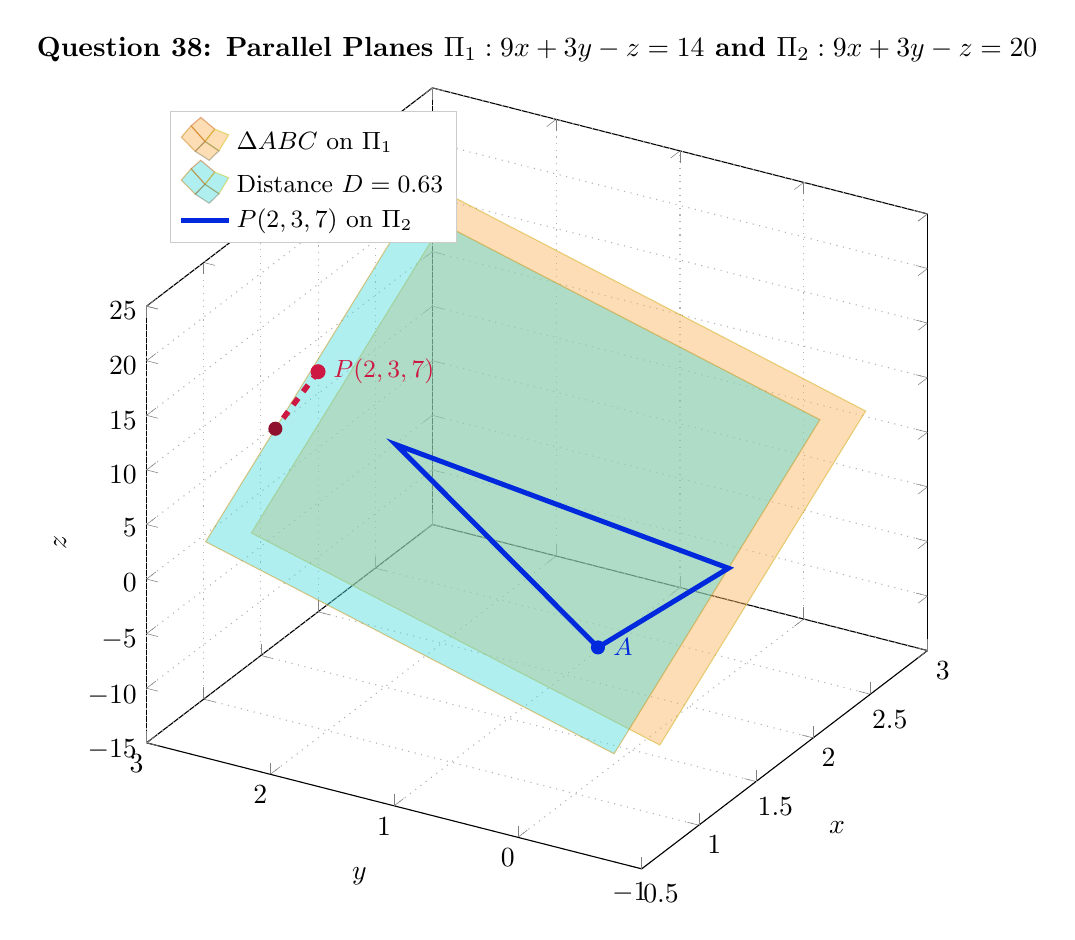
\begin{tikzpicture}
		\begin{axis}[
			width=11.5cm, height=11.5cm,
			view={-60}{30},
			title={\textbf{Question 38: Parallel Planes $\Pi_1 : 9x + 3y - z = 14$ and $\Pi_2 : 9x + 3y - z = 20$}},
			xlabel={$x$}, ylabel={$y$}, zlabel={$z$},
			xmin=0.5, xmax=3.0,
			ymin=-1, ymax=3,
			zmin=-15, zmax=25,
			xtick={0.5, 1.0, 1.5, 2.0, 2.5, 3.0},
			ytick={-1, 0, 1, 2, 3},
			ztick={-15, -10, -5, 0, 5, 10, 15, 20, 25},
			grid=both,
			grid style={dotted, gray!60},
			legend cell align={left},
			legend style={at={(0.03,0.97)}, anchor=north west, font=\small, draw=gray!40}
			]
			% Lower Plane Pi_2: z = 9x + 3y - 20 (orange)
			\addplot3[
			surf, opacity=0.45, fill=planetwo, draw=none,
			domain=1.2:3.0, domain y=-0.5:2.8, samples=2
			] {9*x + 3*y - 20};
			
			% Upper Plane Pi_1: z = 9x + 3y - 14 (cyan)
			\addplot3[
			surf, opacity=0.45, fill=planeone, draw=none,
			domain=0.8:2.6, domain y=-0.5:2.8, samples=2
			] {9*x + 3*y - 14};
			
			% Triangle ABC on Pi_1
			\addplot3[blueedge, line width=1.8pt] coordinates {
				(1.2, 0, -3.2) (1.6, 2, 6.4) (1.8, -0.5, 0.7) (1.2, 0, -3.2)
			};
			\addlegendentry{$\Delta ABC$ on $\Pi_1$}
			
			% Distance segment between planes
			\addplot3[distred, dashed, line width=2pt] coordinates {(2.0, 3.0, 7.0) (1.41, 2.80, 7.07)};
			\addlegendentry{Distance $D = 0.63$}
			
			% Point P(2, 3, 7) on Pi_2
			\addplot3[only marks, mark=*, mark size=2.5pt, distred] coordinates {(2.0, 3.0, 7.0)};
			\addlegendentry{$P(2, 3, 7)$ on $\Pi_2$}
			
			% Endpoint on Pi_1
			\node[circle, fill=distred!70!black, inner sep=1.8pt] at (axis cs:1.41, 2.80, 7.07) {};
			
			% Labels
			\node[right=2pt, font=\small\bfseries, text=distred] at (axis cs:2.0, 3.0, 7.0) {$P(2, 3, 7)$};
			\node[circle, fill=blueedge, inner sep=1.8pt] at (axis cs:1.2, 0, -3.2) {};
			\node[right=2pt, font=\small\bfseries, text=blueedge] at (axis cs:1.2, 0, -3.2) {$A$};
		\end{axis}
	\end{tikzpicture}
\end{document}